\newcommand{\ClassPath}{../../VIU_TFM_LaTeX_template}
\documentclass{\ClassPath/viu-tfm-template}
\usepackage{multicol}

\definecolor{maincolor}{HTML}{f25416}

%--------------------------------------------------------------------------
% Definiciones necesarias Modifica con tus datos
%--------------------------------------------------------------------------
\def\nombre{Gómez Olivencia, Rubén}
\def\dni{78910013-A}
\def\titulo{Creando una calculadora \linebreak\linebreak con Kotlin para Android}
\def\titulacion{Máster Universitario en Desarrollo de Aplicaciones y Servicios Web}
\def\curso{2022-2023}

%Los siguientes son opcionales: si no se ponen, la portada cambia un poco. Ideal para escribir artículos/trabajos cortos
\def\dirige{}
\def\convocatoria{}
\def\asignatura{Programación en dispositivos móviles (wearables)}


% importar fichero de Bibliografía
%\addbibresource{Actividad_1.bib}

\begin{document}
    \graphicspath{{../../VIU_TFM_LaTeX_template/}}

    \coverpage

    \tableofcontents

\chapter{Introducción}

Dentro de la programación móvil existen dos grandes sistemas operativos que abarcan casi toda la cuota de mercado actual: Android e iOS. El primero, bajo el paraguas de Google, y con kernel Linux, puede ser programado bajo cualquier sistema operativo, mientras que para el segundo se requiere de un ecosistema basado en MacOS.

A la hora de aprender un nuevo lenguaje de programación, o un \textit{framework} basado en él, la mejor manera es hacerlo creando un proyecto real. El proyecto a crear no tiene por qué ser complejo, pero sí que debe  tener unas funcionalidades básicas que permitan aprender ciertas características del lenguaje.

En esta documentación se va a explicar los pasos realizados para la creación de una aplicación que funcionará en el sistema operativo Android y creada bajo el lenguaje de programación Kotlin.


\chapter{Requisitos del proyecto}

Tal como se ha dicho, la mejor manera de aprender es crear una aplicación sencilla, en este caso una calculadora. Que sea sencilla no quita que deba cumplir con una serie de requisitos para poder satisfacer la adquisición de unos conocimientos básicos.

Los requisitos establecidos son:

\begin{itemize}
    \item La calculadora contará con al menos dos operaciones (sumar y restar).
    \item La entrada de números será a través de botones correspondientes a los dígitos.
    \item La interfaz se debe adaptar al tamaño de la pantalla.
    \item La aplicación se deberá visualizar de forma diferente si se encuentra en modo vertical o horizontal.
    \item La aplicación estará en al menos dos idiomas.
    \item A través de un botón el resultado se mostrará en otro \textit{Activity}.
    \item En ese nuevo Activity, la aplicación permitirá compartir el resultado utilizando otras aplicaciones del sistema.
\end{itemize}


\chapter{Creación del proyecto}

Para la creación del proyecto se ha hecho uso del entorno de desarrollo \href{https://developer.android.com/studio/}{Android Studio}, que es el IDE oficial que nos permite programar teniendo todos los recursos necesarios.

Por otro lado, se ha hecho uso del lenguaje de programación \href{https://kotlinlang.org/}{Kotlin}, ya que desde el año 2019 Google lo ha puesto como el lenguaje de programación preferido a la hora de realizar los desarrollos para la plataforma Android.

A continuación se detallan los aspectos más destacados del proyecto.

\section{Diseño del interfaz}
Tal como se ha visto en los requisitos, uno de ellos es que la aplicación debe de tener visualizaciones distintas dependiendo de si el móvil está en modo vertical o en modo horizontal.

Para la creación de la aplicación primero se creó el diseño en modo vertical, siguiendo el aspecto visual clásico que suelen tener la gran mayoría de las aplicaciones de este tipo.

{
    \begin{minipage}{0.3\linewidth}
        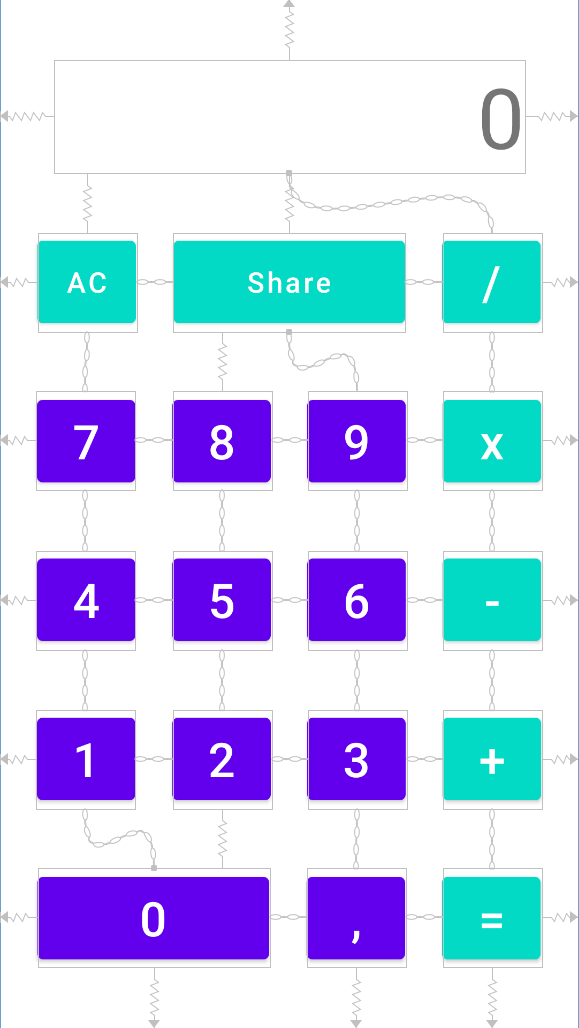
\includegraphics[frame,width=\linewidth]{img/portrait.png}
    \end{minipage}
    \hfill
    \begin{minipage}{0.65\linewidth}
        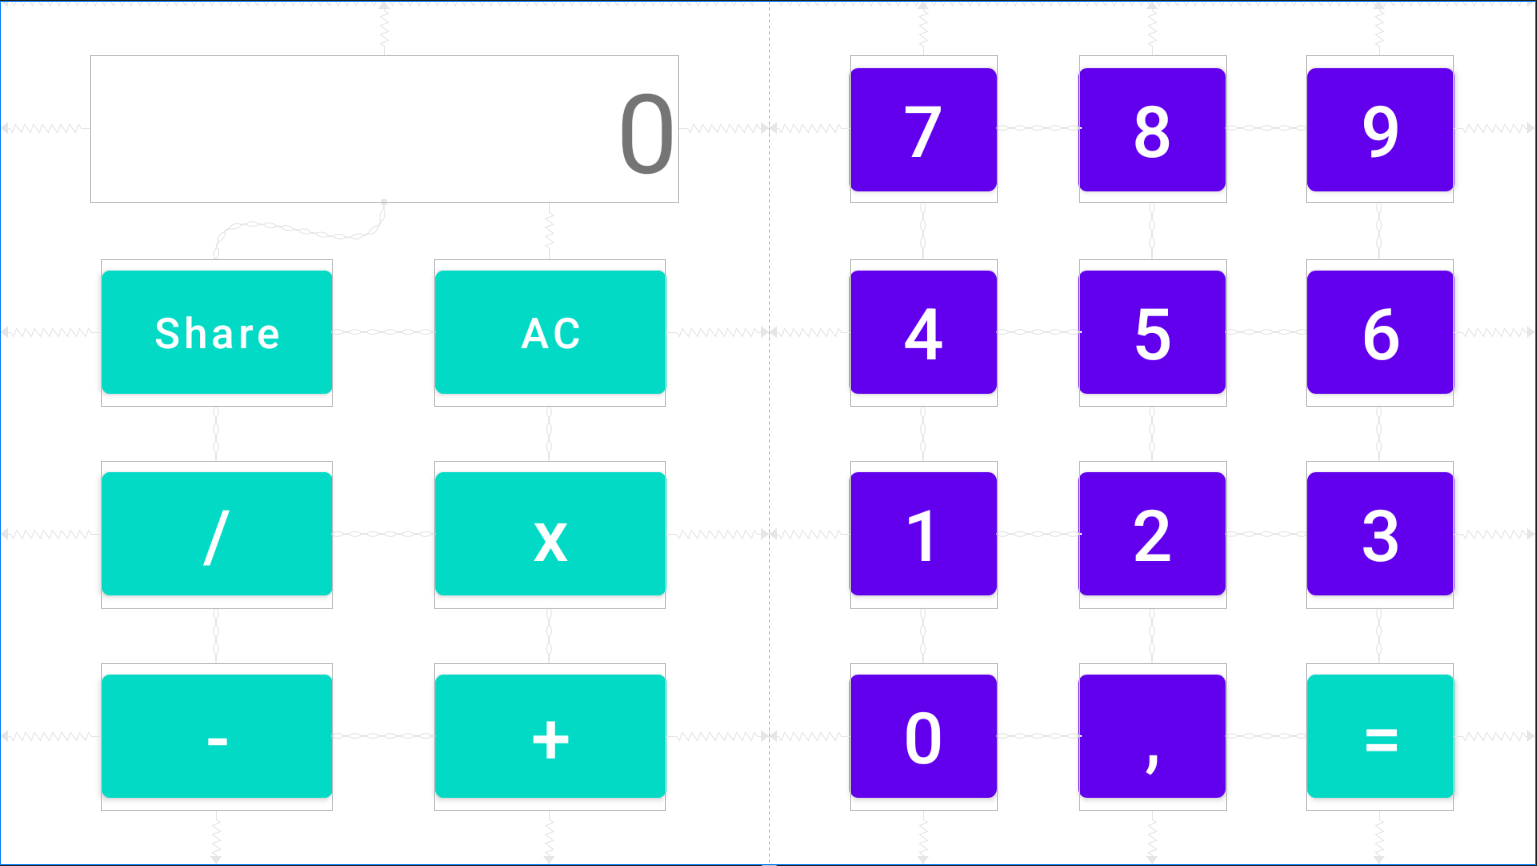
\includegraphics[frame,width=\linewidth]{img/landscape.png}
    \end{minipage}
}

Para la correcta colocación de los botones, y que se ajusten en todo momento al interfaz (sin importar el tamaño de la pantalla), se ha hecho uso de las denominadas “cadenas”, tanto en sentido horizontal como vertical.

De esta manera, los botones tienen unas relaciones entre sí y con los bordes de la pantalla que hace que se coloquen de manera relativa al tamaño de la pantalla, quedando de la siguiente manera:


{
    \begin{minipage}{0.4\linewidth}
        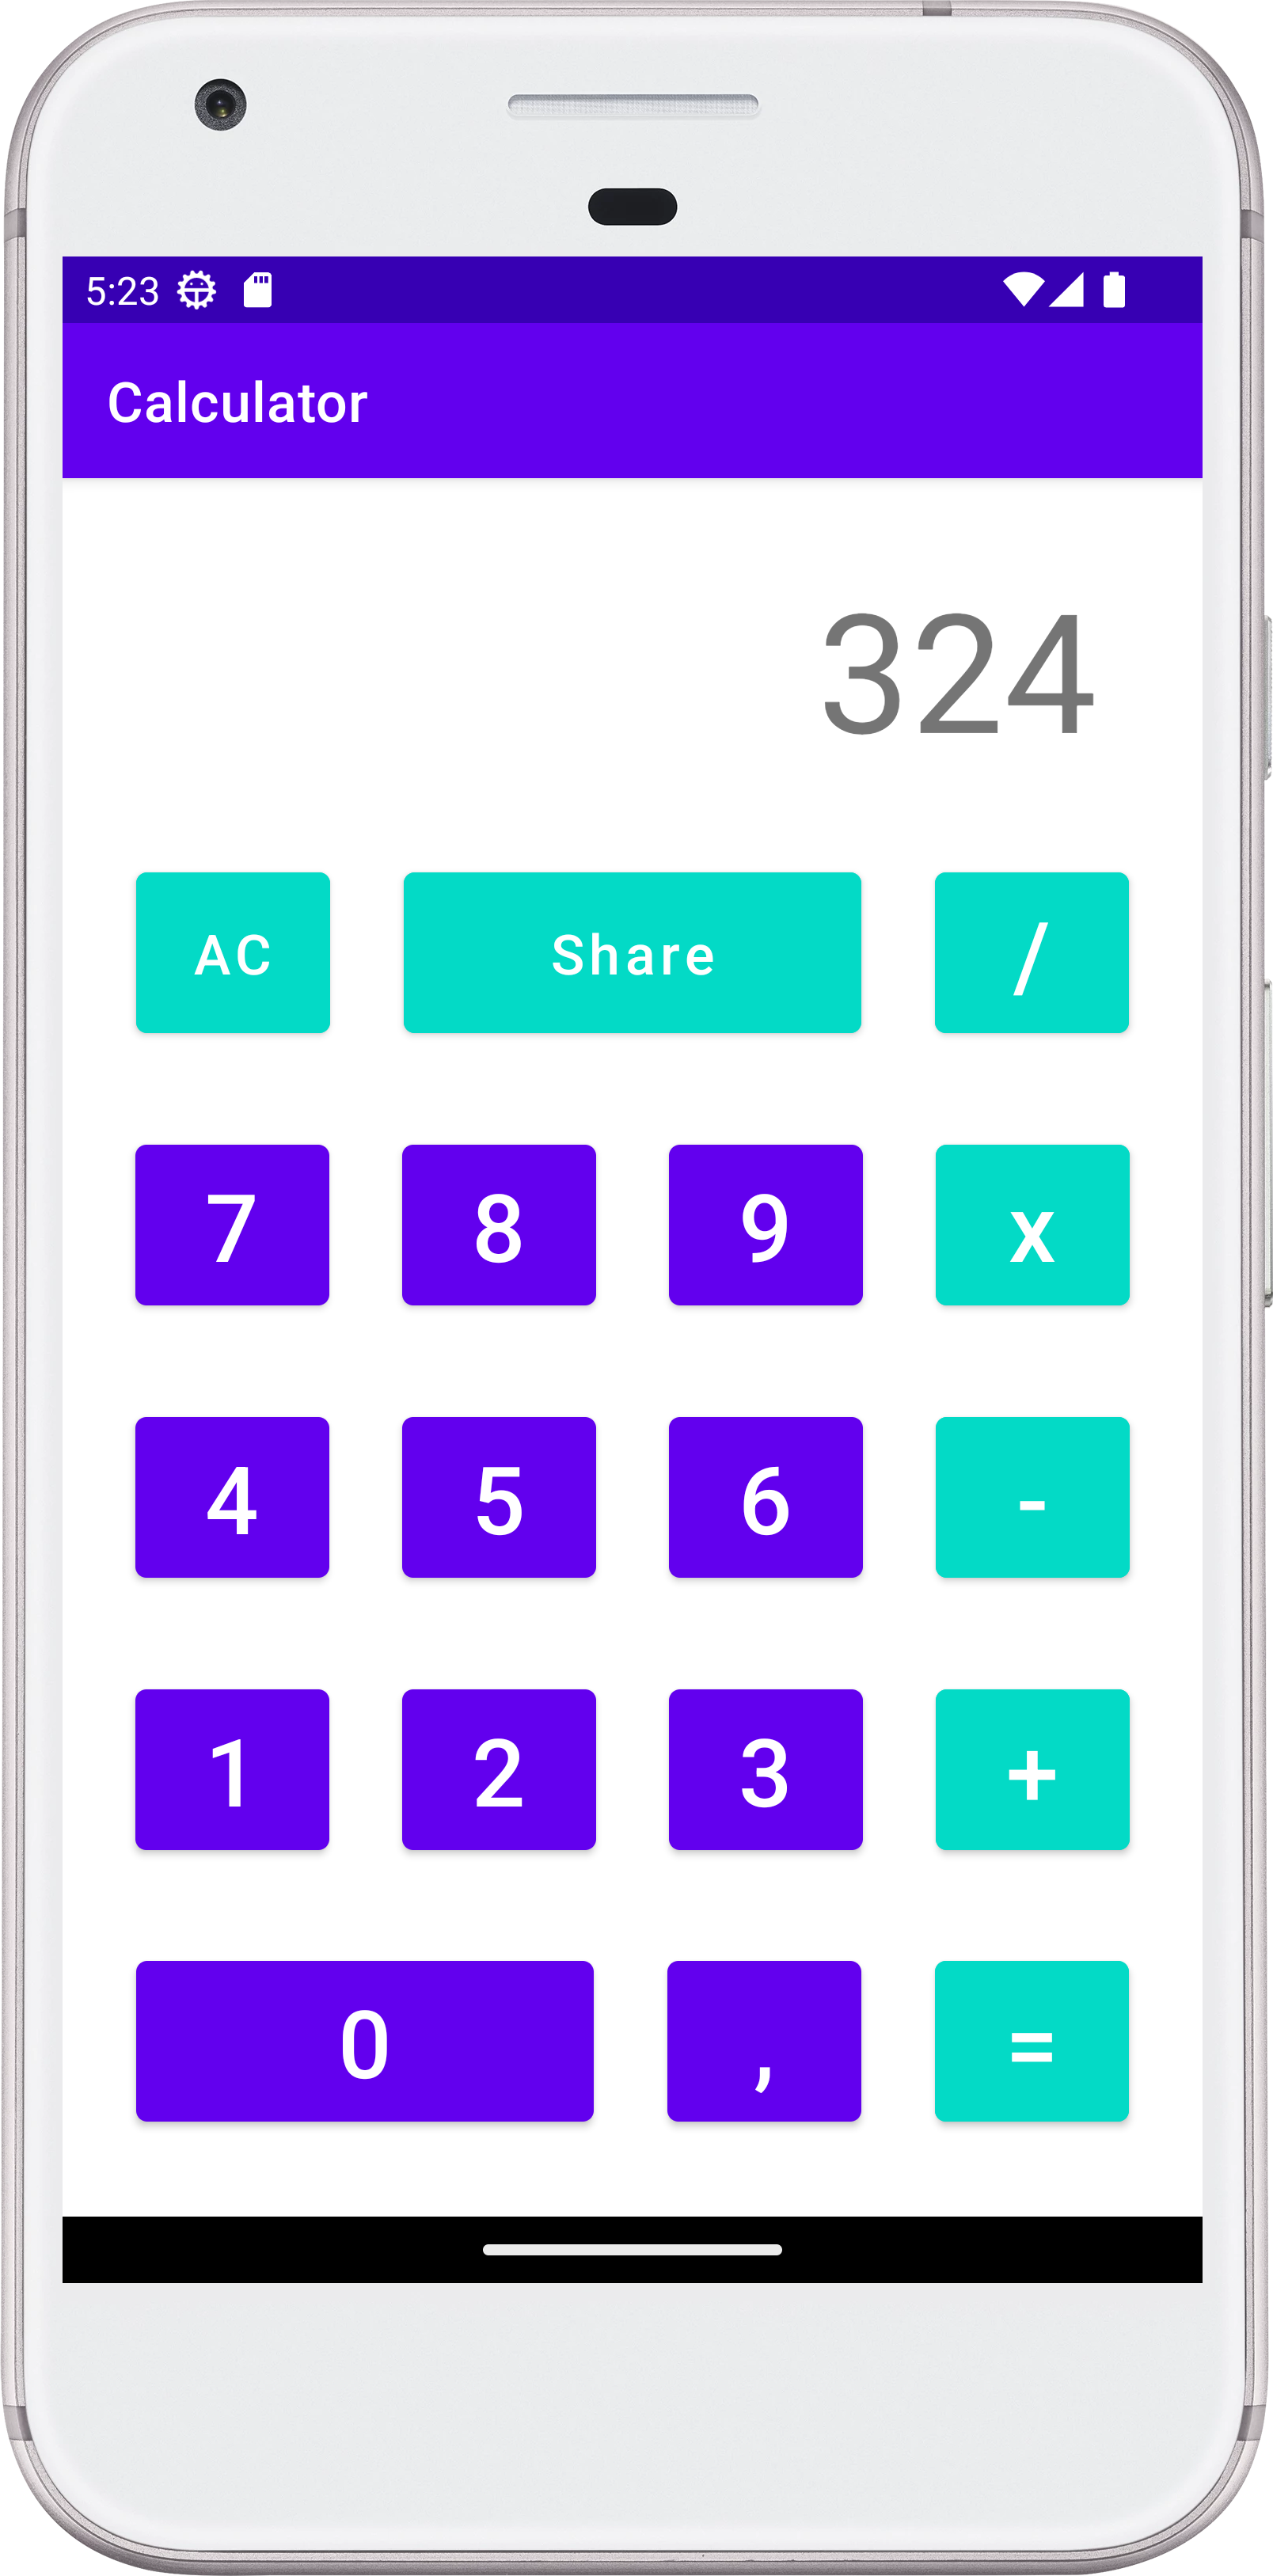
\includegraphics[width=\linewidth]{img/phone1.png}
    \end{minipage}
    \hfill
    \begin{minipage}{0.4\linewidth}
        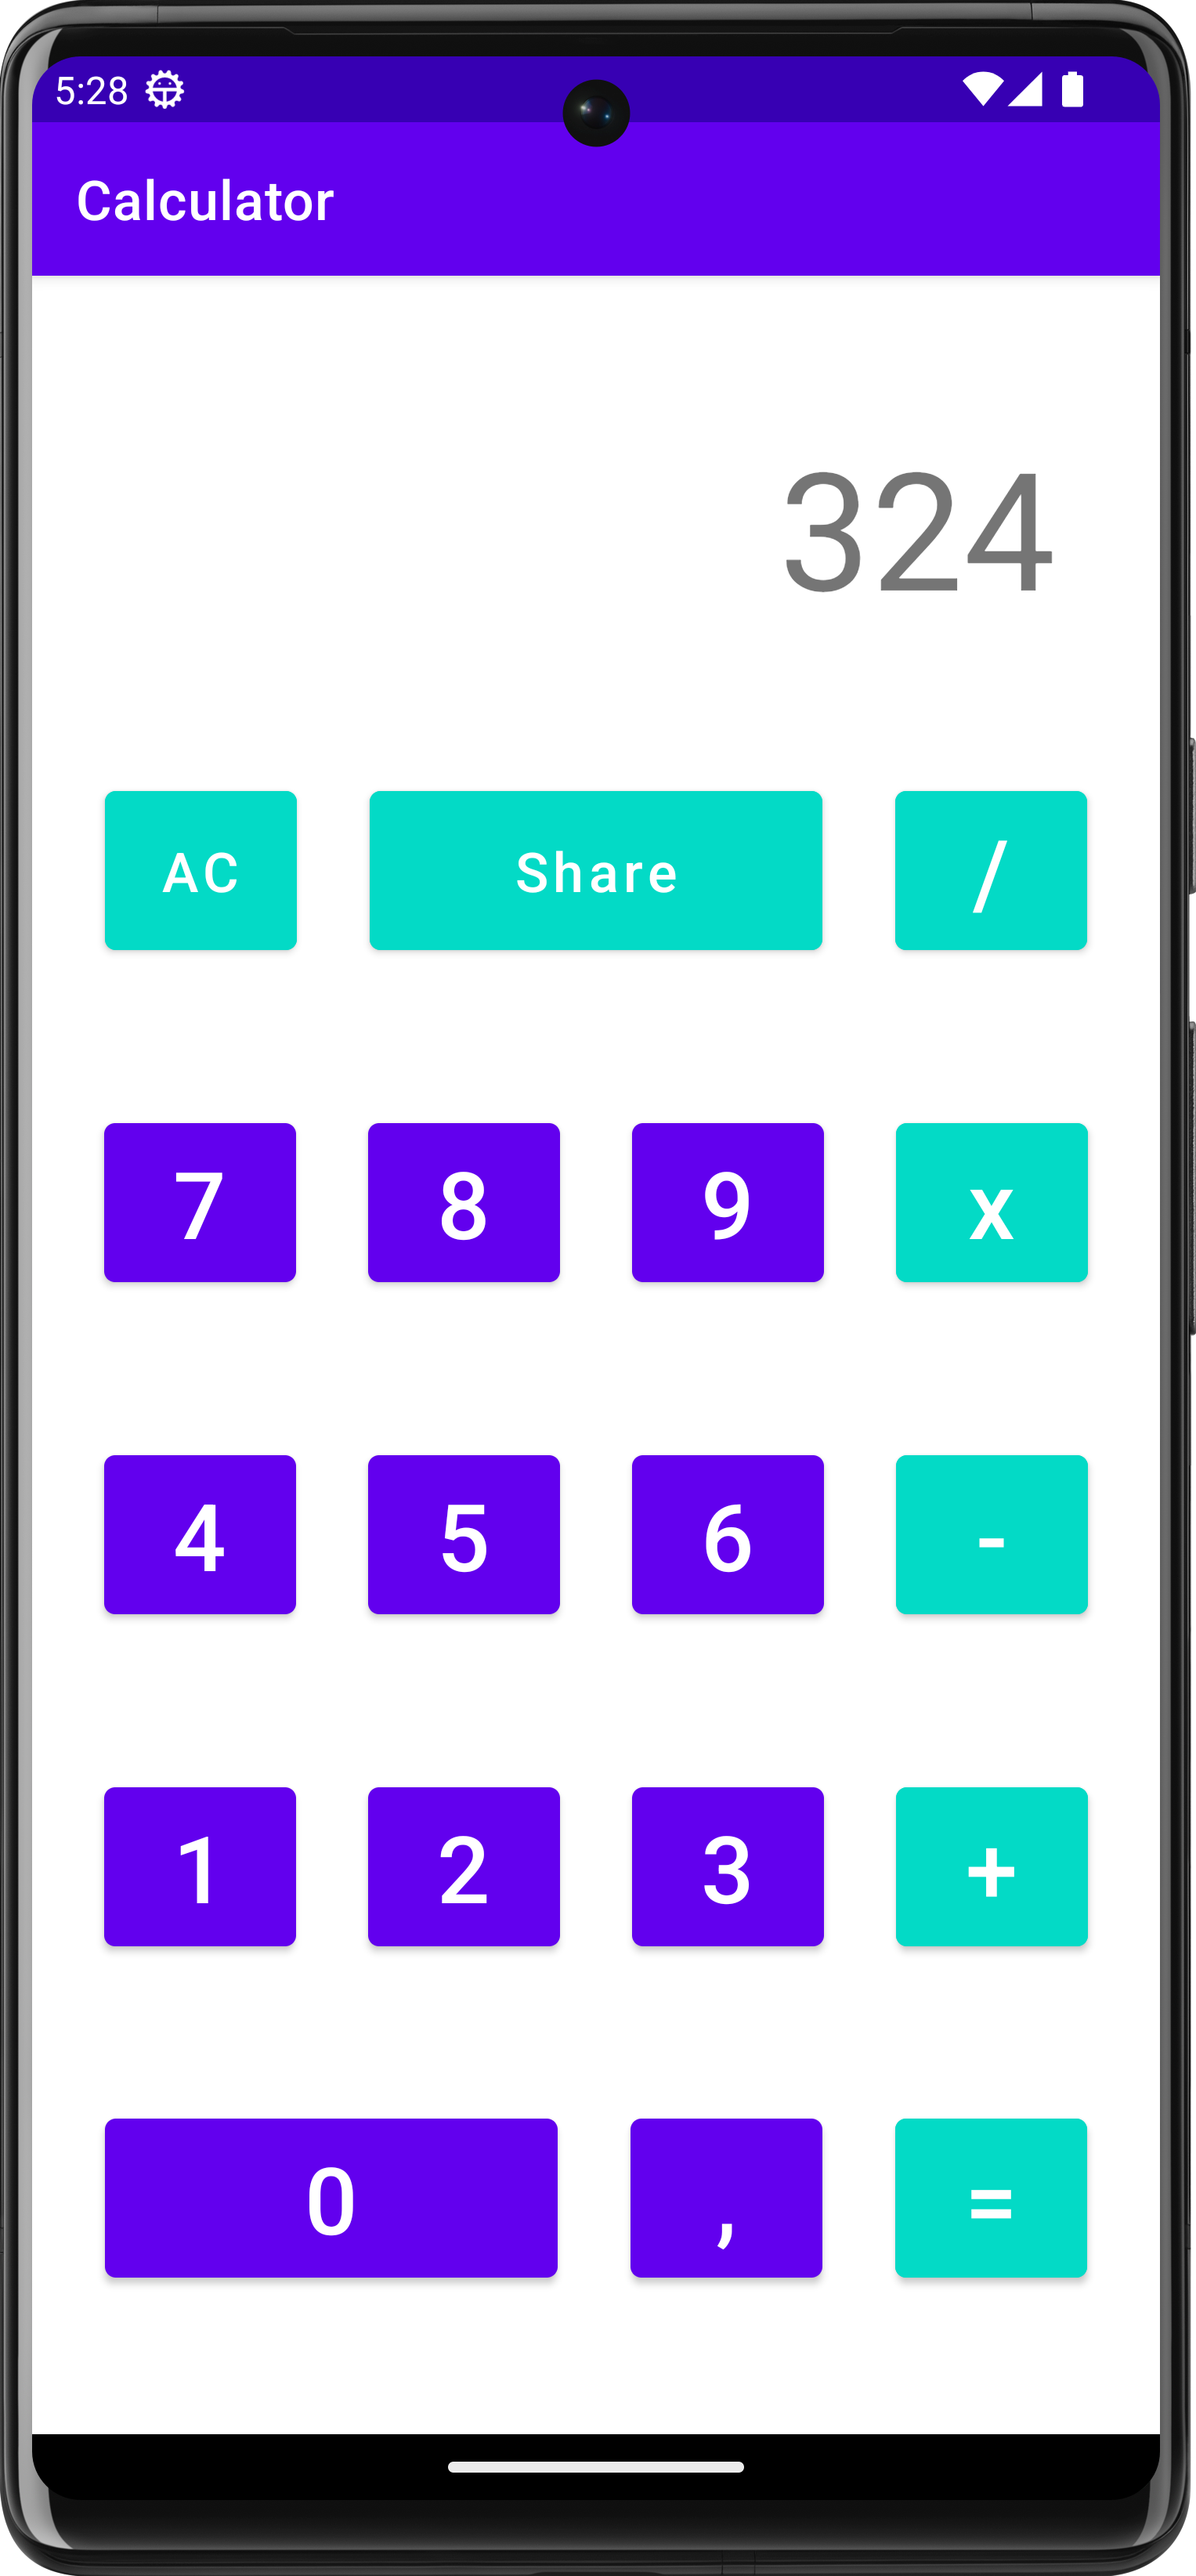
\includegraphics[width=\linewidth]{img/phone2.png}
    \end{minipage}
}


Para el modo apaisado, se ha seguido la misma filosofía, pero esta vez se ha utilizado también una “guía de línea vertical” (\textbf{\textit{vertical guideline}}) colocada en el centro de la pantalla.


\begin{mycode}{Parte del código XML del Activity en modo landscape}{XML}{}
<androidx.constraintlayout.widget.Guideline
    android:id="@+id/guideline3"
    android:layout_width="wrap_content"
    android:layout_height="wrap_content"
    android:orientation="vertical"
    app:layout_constraintEnd_toEndOf="parent"
    app:layout_constraintGuide_percent="0.5"
    app:layout_constraintStart_toStartOf="parent" />
\end{mycode}

Esta guía nos permite que los \textit{constraints} en lugar de ir hasta el borde de la pantalla, se conecten a esta guía. De esta manera, en el modo apaisado se puede diferenciar entre el lado izquierdo (con el resultado y los botones de acción y operaciones) y el lado derecho (con los botones de los números y el igual).

Por último, para que exista una diferenciación, los botones de acción (ya sea de operaciones aritméticas, igual, reset y compartir) se les ha dado un color denominado “\textbf{\textit{design\_default\_color\_secondary}}”, que es distinto a los botones numéricos.


\section{Lógica de la aplicación}
Una vez realizado el interfaz, es el momento de hacer que los botones cumplan su función aplicando la lógica que deben de tener para que el proyecto cumpla con su función principal: calcular.

A la hora de programar, se ha tratado de que el código sea lo más modular posible y eficaz, para que cualquier posible cambio futuro sea sencillo de realizar.

Por ejemplo, a la hora de implementar las acciones sobre los botones de los números, una vez obtenido los objetos, en lugar de ir uno a uno, se ha creado un array que se ha recorrido en un bucle para configurarles la acción \textbf{\textit{setOnClickListener}}.

\begin{mycode}{Bucle para la acción \textbf{setOnClickListener} de los números}{kotlin}{}
// onclick actions for numbers
val numbers = arrayOf(button0,button1,button2,button3,button4,
button5,button6,button7,button8,button9)
for ((index, element) in numbers.withIndex()) {
    element.setOnClickListener {
        // ...
        tresult.text = tresult.text.toString() + index.toString()
    }
}
\end{mycode}

Por otro lado, a la hora de realizar las operaciones matemáticas implementadas (sumar, restar, multiplicar y dividir) se ha hecho uso de dos variables de tipo \textbf{Double}, que junto con la operación pulsada, al darle al botón “igual”, se llama a la siguiente función:

\begin{mycode}{Función que determina la operación a realizar}{kotlin}{}
// check which operation must be done
fun do_operation(operation:String,n1:Double,n2:Double):Double{
    when (operation){
        "+" -> return sumar(n1,n2)
        "-" -> return restar(n1,n2)
        "*" -> return multiplicar(n1,n2)
        "/" -> return dividir(n1,n2)
        else -> return 0.0 //never
    }
}
\end{mycode}

Tal como se puede ver, a su vez llama a otras funciones que también han sido creadas para la aplicación.

%\subsection{Formato de texto}
% TODO: encontrado bug mientras escribía esto.
%
%Debido al uso de \textbf{Double} como resultado, el número que se puede llegar a obtener es muy grande, y por tanto cabe la posibilidad de que no se visualice de manera correcta. Es por eso que el en la configuración del \textit{TextView} se han añadido los siguietnes parámetros de configuración:
%
%\begin{mycode}{Función que determina la operación a realizar}{kotlin}{}
%<TextView
%    ...
%    android:autoSizeMaxTextSize="60sp"
%    android:autoSizeMinTextSize="10sp"
%    android:autoSizeTextType="uniform"
%    android:textSize="60sp" />
%\end{mycode}
%
%Con ellos se indica el tamaño máximo del texto que contiene el \textit{TextView} y el tamaño mínimo, que se ajusta de manera automática y de manera uniforme, dando como resultado las siguientes posibles vistas, dependiendo del número de digitos del resultado:



\section{Idiomas de la aplicación}
Otro aspecto que se ha tenido en cuenta ha sido la internacionalización de la aplicación. Los pocos textos que contiene, se han generado en tres idiomas: inglés, castellano y euskera.

Para ello, se han generado los textos a través del \textit{\textbf{Translations Editor}}, que por debajo hace uso de un fichero en formato XML para cada idioma. Luego cada \textit{TextView} hace referencia a la clave del texto asociado.

{
\begin{minipage}{0.32\linewidth}
    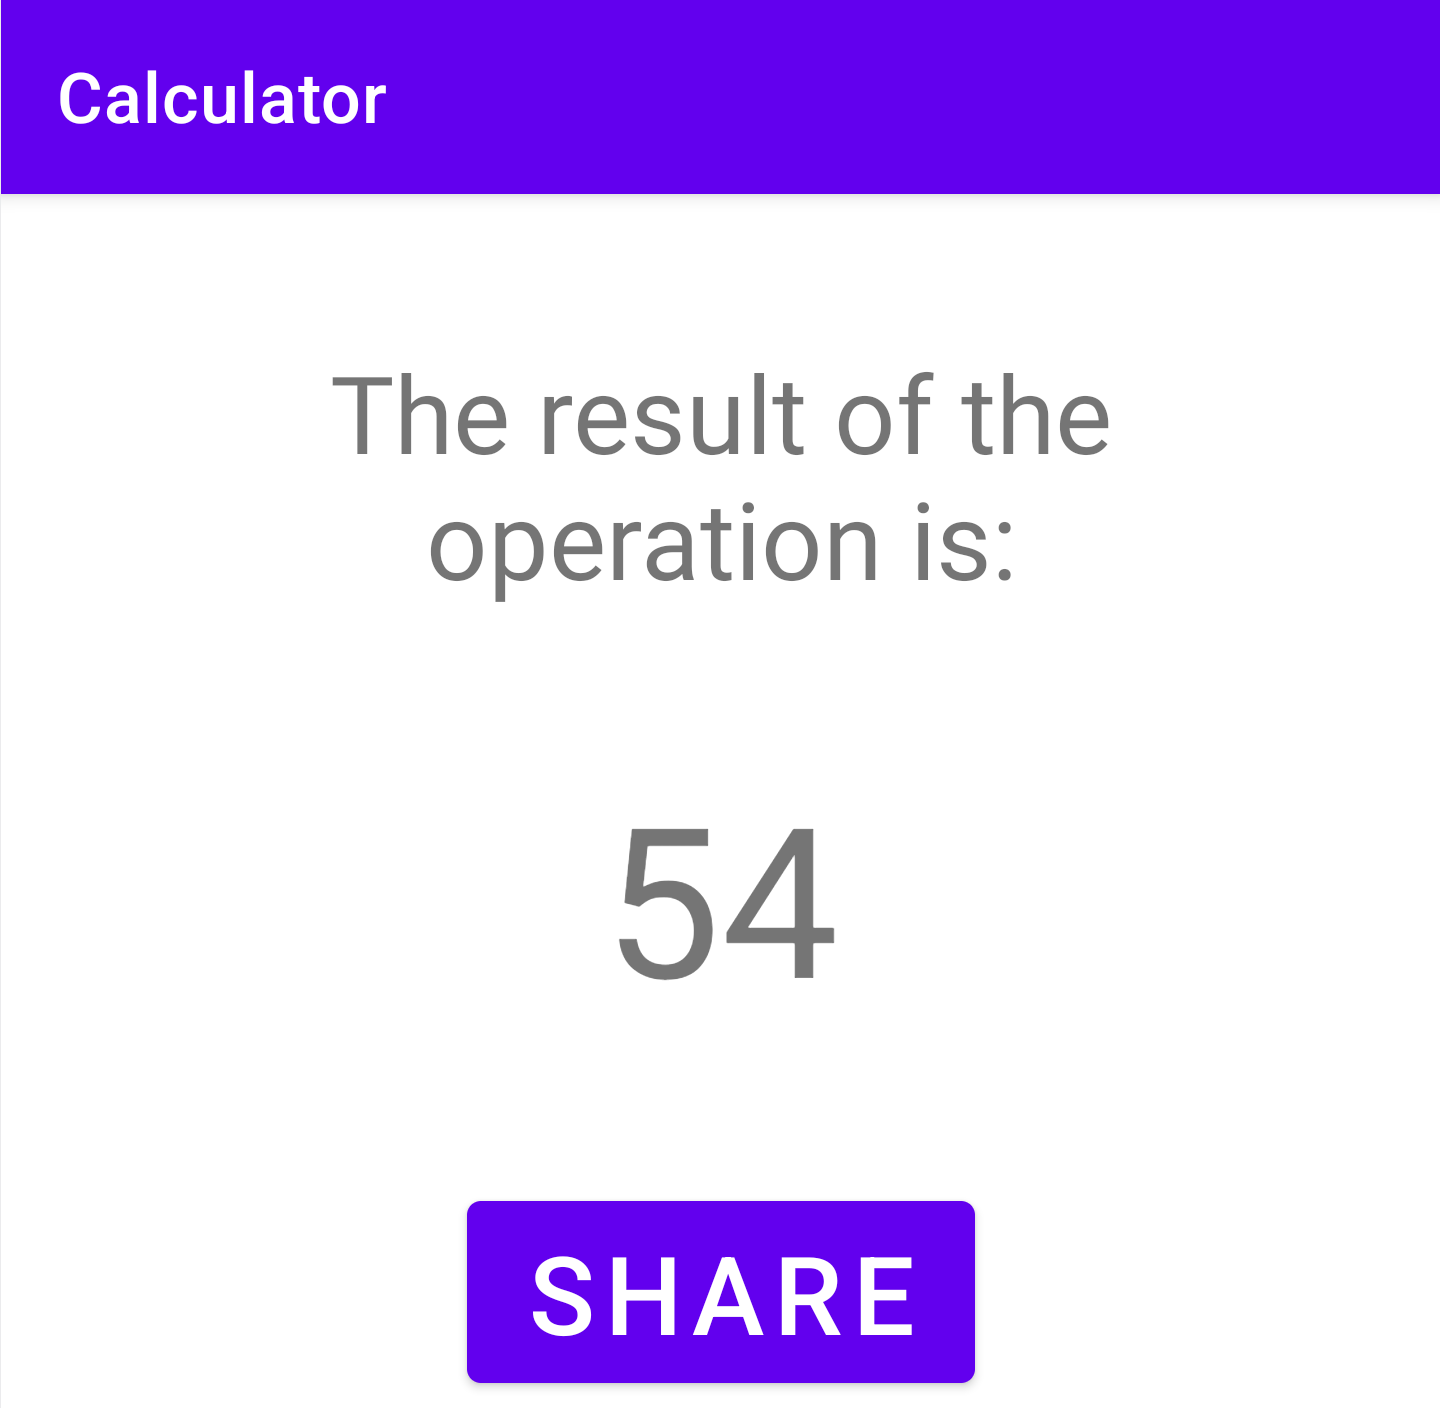
\includegraphics[frame,width=\linewidth]{img/english.png}
\end{minipage}
\hfill
\begin{minipage}{0.32\linewidth}
    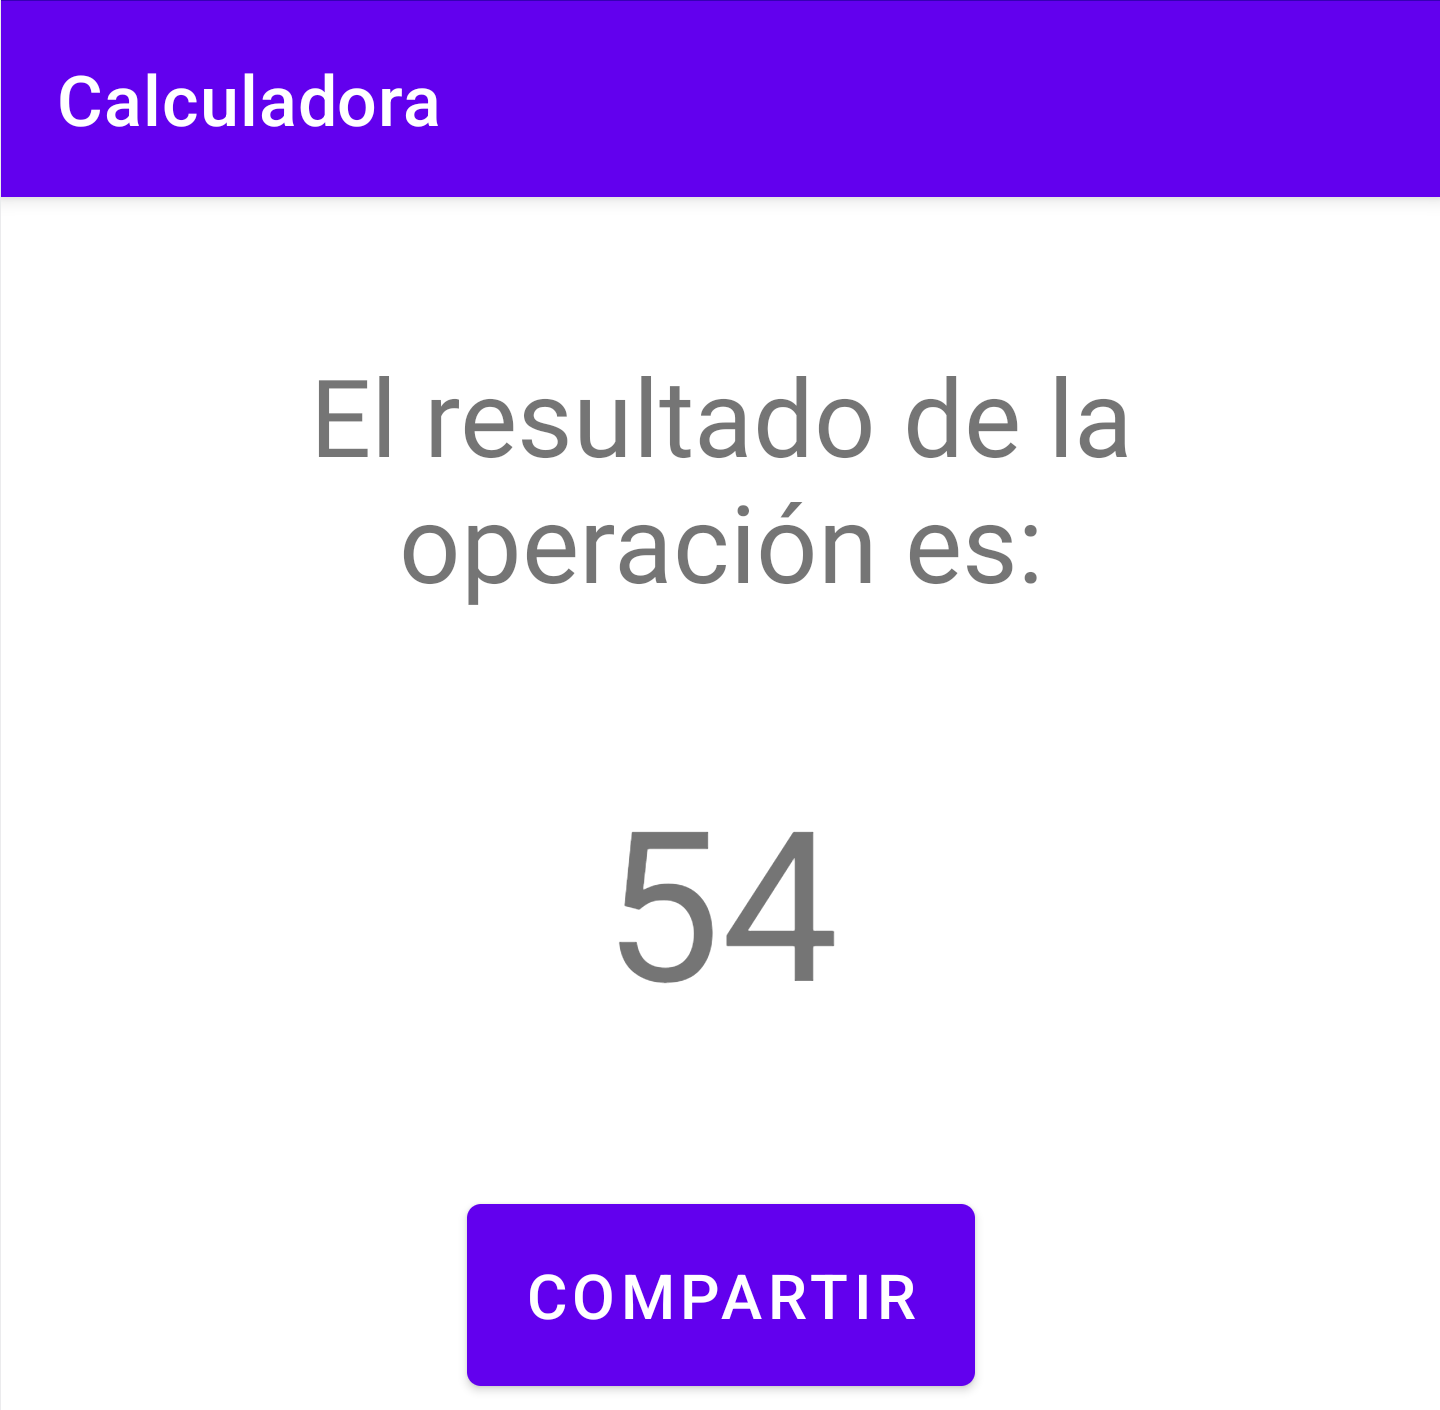
\includegraphics[frame,width=\linewidth]{img/castellano.png}
\end{minipage}
\hfill
\begin{minipage}{0.32\linewidth}
    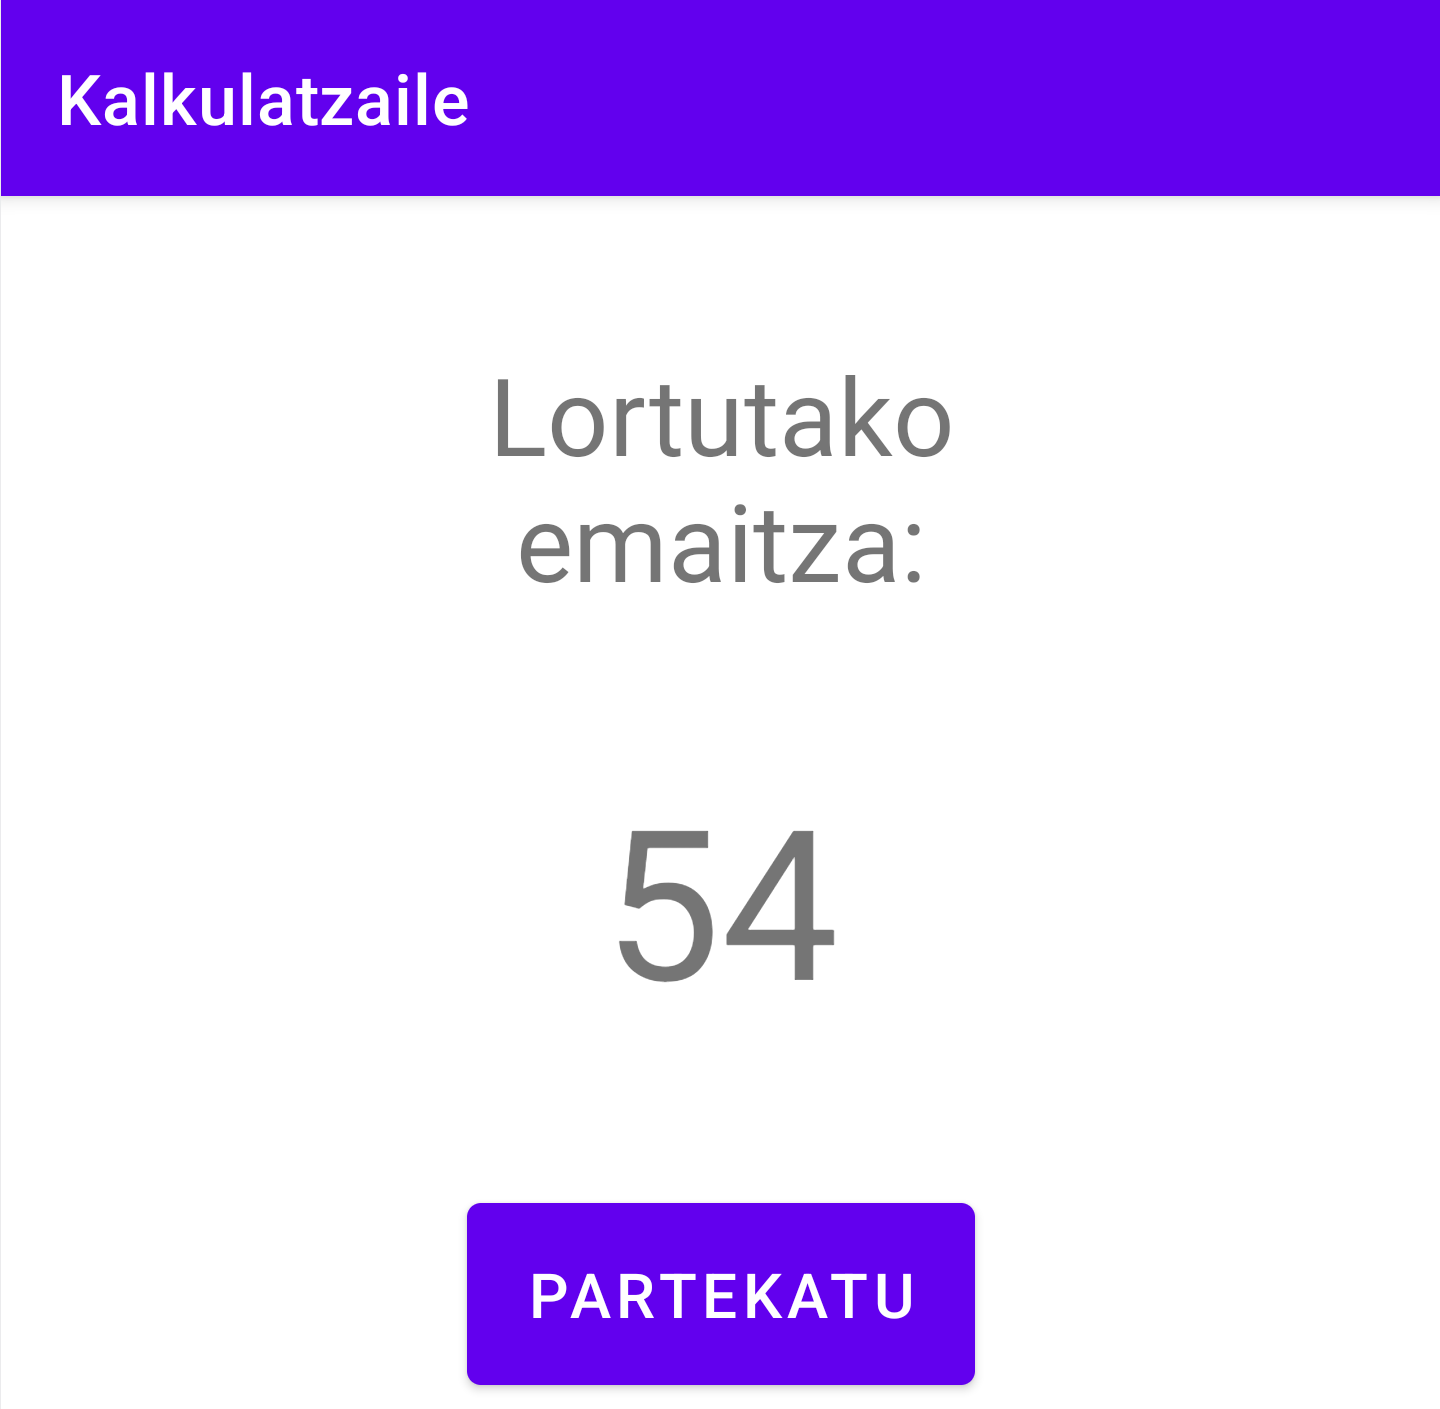
\includegraphics[frame,width=\linewidth]{img/euskara.png}
\end{minipage}

}

De esta manera, al cambiar el terminal de idioma, la aplicación detectará el cambio y obtendrá los textos para el idioma seleccionado, y se visualiza en dicho idioma, como se puede ver en las imágenes anteriores.


\section{Guardar estados al girar la pantalla}

Por cómo funcionan los ciclos de vida de los Activity, al girar la pantalla el Activity se reinicia, y eso hacía que se perdiese el resultado y la operación que se estaba realizando en el momento del giro.

Para evitar eso, se han creado dos funciones para guardar el estado y posteriormente restaurarlo.

\begin{mycode}{Función que guarda el estado}{kotlin}{}
// Function to save the Instance state
override fun onSaveInstanceState(outState: Bundle) {
    super.onSaveInstanceState(outState)
    outState.putDouble("result",result)
    outState.putDouble("number",number)
    outState.putString("operation",operation)
    outState.putBoolean("clean",clean)
}
\end{mycode}

La función guarda el estado del resultado actual, la operación que se está realizando, el número que realiza la operación y si hay que “limpiar” el resultado. La función de restauración recupera esos estados.

\section{Navegación entre \textit{activities}}

Para realizar otro de los requisitos exigidos era necesario crear un segundo Activity, en el que visualizaremos el resultado de la operación. En este Activity tendremos un botón que nos permite compartir el resultado con otras aplicaciones del sistema.


Para enviar el resultado al segundo Activity se hace a través del evento \textbf{setOnClickListener} que pertenece al botón “bshare” de la primera pantalla de la calculadora:

\begin{mycode}{Evento onClick del botón share}{kotlin}{}
// share result into Result-Activity
bshare.setOnClickListener {
    val intent = Intent(this, ResultActivity::class.java)
    intent.putExtra(ResultActivity.RESULT, format_result(result))
    startActivity(intent)
}
\end{mycode}


El Activity que recibe el resultado se llama “\textbf{activity\_result}, en el cual sólo aparece una frase, el resultado obtenido a través del evento anterior y el botón de compartir.

\begin{center}
    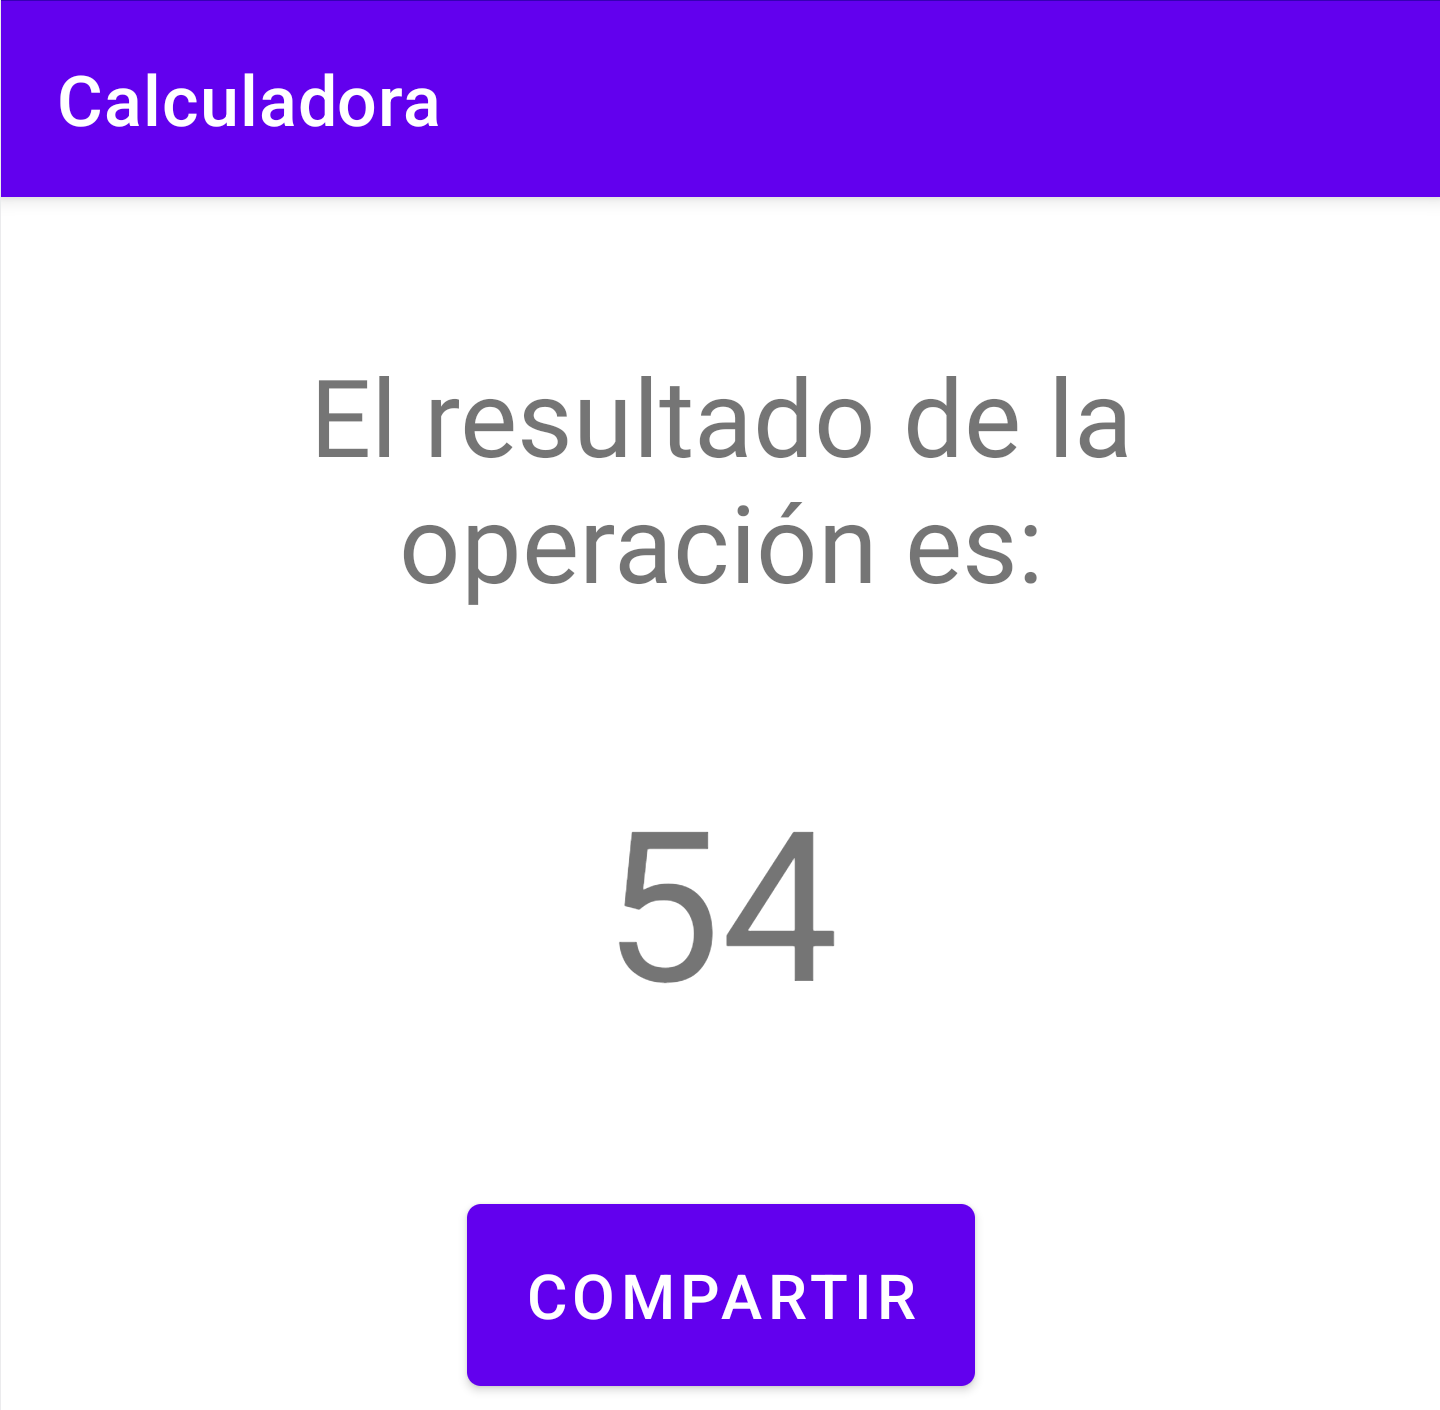
\includegraphics[frame,width=0.33\linewidth]{img/castellano.png}
\end{center}


\section{Compartir resultado}

Al dar al botón de compartir (con el texto en el idioma con el que está configurado el terminal) de la imagen del apartado anterior, nos mostrará el \textit{pop-up} de la siguiente imagen.

\begin{center}
    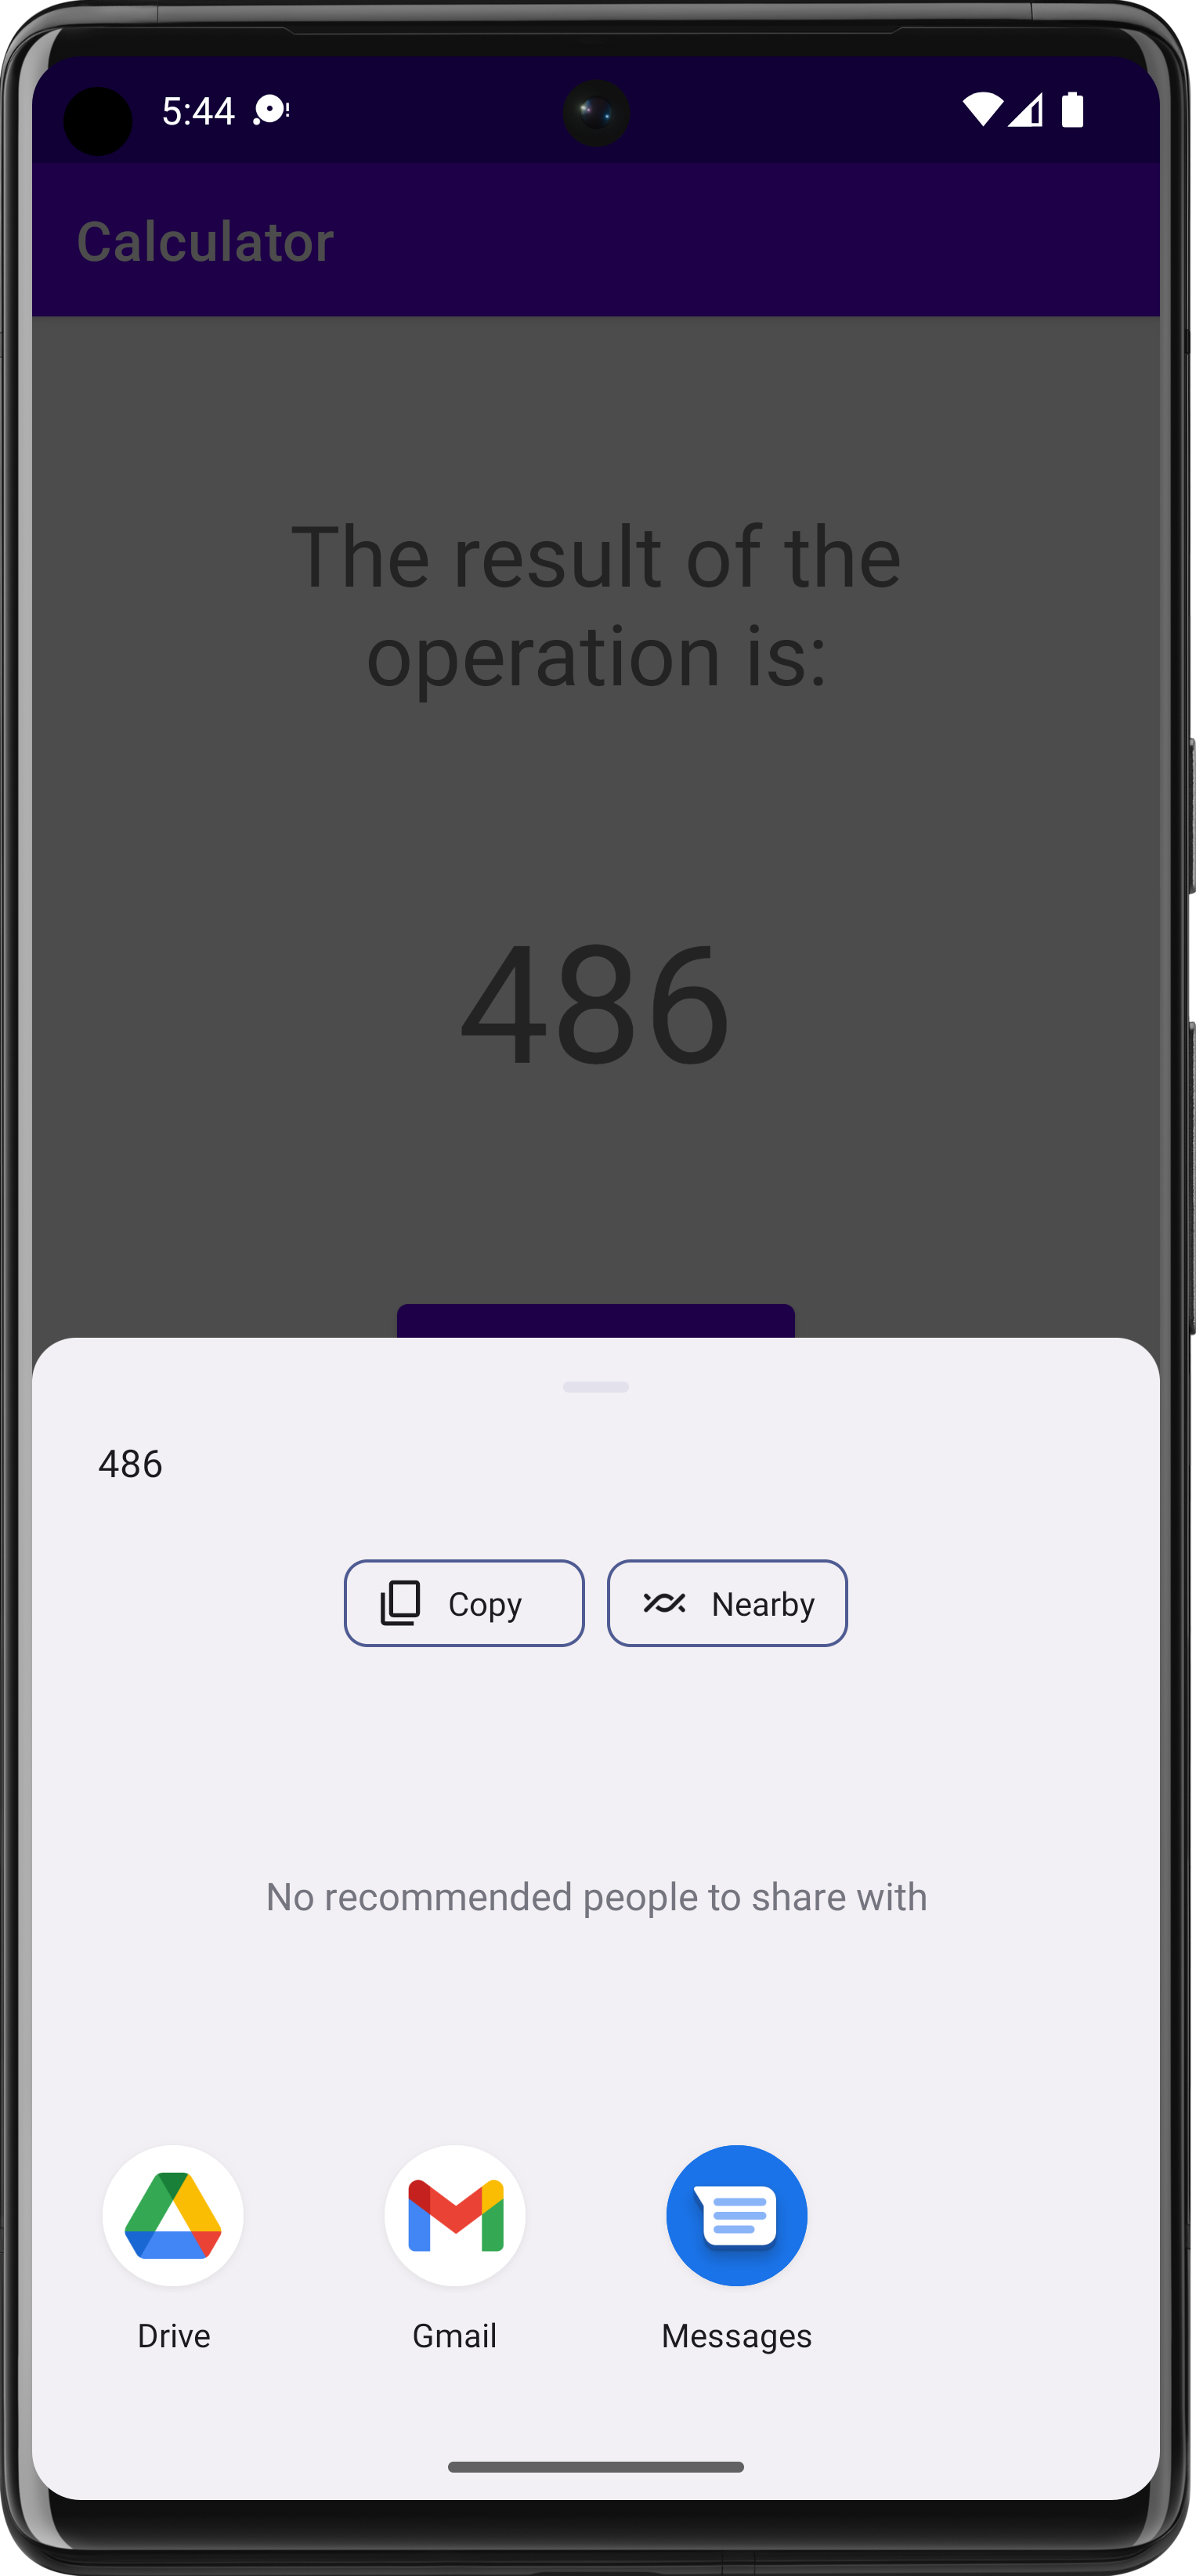
\includegraphics[width=0.4\linewidth]{img/share.png}
\end{center}



Para que aparezca el \textit{pop-up} de aplicaciones en este segundo Activity, al dar al botón con el texto “compartir”, se realiza la siguiente ejecución:

\begin{mycode}{Llamada al pop-up de aplicaciones}{kotlin}{}
// share button
val bshare = findViewById<Button>(R.id.bshare_result)

val sendIntent = Intent().apply {
    action = Intent.ACTION_SEND
    putExtra(Intent.EXTRA_TEXT,result)
    // if the type is "text/plain" will not show all apps.
    type = "text/plain"
}

val shareIntent = Intent.createChooser(sendIntent,null)

bshare.setOnClickListener {
    if (sendIntent.resolveActivity(packageManager) != null) {
        startActivity(shareIntent)
    }
}
\end{mycode}

Lo que indica el código fuente es que cuando se pulsa el botón, comienza el evento “onClick” que lanzará un “\textbf{Intent}” que va a realizar la acción “\textit{ACTION\_SEND}”, con el \textit{EXTRA\_TEXT}” que tiene el resultado, que es del tipo “text/plain”.

Dependiendo del tipo que se ponga, en el \textit{pop-up} aparecerán distintas aplicaciones. El tipo hace referencia a los \href{https://en.wikipedia.org/wiki/Media_type}{MIME types}, y Android lo tiene en cuenta a la hora de qué aplicaciones mostrar.


\chapter{Conclusiones}

Aunque el proyecto de una calculadora \textit{a priori} no parece complejo, con lo realizado se ha podido aprender los fundamentos básicos para poder hacer aplicaciones más complejas: uso de varios Activity, envío de información entre ellas, guardar estados al haber eventos, internacionalización...

Con ello, también se ha visto el potencial que tiene Kotlin, un lenguaje de programación moderno que junto con el IDE Android Studio hace que realizar una aplicación móvil resulte sencillo y agradable.


\end{document}
